%%%%%%%%%%%%%%%%%%%%%%%%%%%%%%%%%%%%%%%%%
% Beamer Presentation
% Pulse Width Modulation on Firebird V
% Author: Vibhu Mishra (e-Yantra Team)
% Reference: www.LaTeXTemplates.com Version 1.0 (10/11/12)
%
%%%%%%%%%%%%%%%%%%%%%%%%%%%%%%%%%%%%%%%%%

%----------------------------------------------------------------------------------------
%	PACKAGES AND THEMES
%----------------------------------------------------------------------------------------
		
\documentclass[table,10pt,red]{beamer}	% First line -- Define document class as Beamer which is used for creating presentation using Latex
\setbeamercolor{alerted text}{fg=blue} 	% Sets color of highlighted text during presentation.  
 

% The Beamer class comes with a number of default slide themes
% which change the colors and layouts of slides. Below this is a list
% of all the themes, uncomment each in turn to see what they look like.

%\usetheme{default}
%\usetheme{AnnArbor}
%\usetheme{Antibes}
%\usetheme{Bergen}
%\usetheme{Berkeley}
\usetheme{Berlin}		%used theme in present documents.
%\usetheme{Boadilla}
%\usetheme{CambridgeUS}
%\usetheme{Copenhagen}
%\usetheme{Darmstadt}
%\usetheme{Dresden}
%\usetheme{Frankfurt}
%\usetheme{Goettingen}
%\usetheme{Hannover}
%\usetheme{Ilmenau}
%\usetheme{JuanLesPins}
%\usetheme{Luebeck}
%\usetheme{Madrid}
%\usetheme{Malmoe}
%\usetheme{Marburg}
%\usetheme{Montpellier}
%\usetheme{PaloAlto}
%\usetheme{Pittsburgh}
%\usetheme{Rochester}
%\usetheme{Singapore}
%\usetheme{Szeged}
%\usetheme{Warsaw}

% As well as themes, the Beamer class has a number of color themes
% for any slide theme. Uncomment each of these in turn to see how it
% changes the colors of your current slide theme.

%\usecolortheme{albatross}
%\usecolortheme{beaver}
%\usecolortheme{beetle}
%\usecolortheme{crane}
%\usecolortheme{dolphin}
%\usecolortheme{dove}
%\usecolortheme{fly}
%\usecolortheme{lily}
%\usecolortheme{orchid}
%\usecolortheme{rose}
%\usecolortheme{seagull}
%\usecolortheme{seahorse}
%\usecolortheme{whale}
%\usecolortheme{wolverine}

%\setbeamertemplate{footline} % To remove the footer line in all slides uncomment this line
%\setbeamertemplate{footline}[page number] % To replace the footer line in all slides with a simple slide count uncomment this line

%\setbeamertemplate{navigation symbols}{} % To remove the navigation symbols from the bottom of all slides uncomment this line
%}

%------------------------------------------------------------------------------------------
%	\usepackage is required for including various features like images, table, references etc.
%	Packages must be installed before using. These can be istalled through package manager. 
%   Various packages have dependencies and for using such packages all dependent packages must be used. 
%-----------------------------------------------------------------------------------------
\usepackage{beamerthemeshadow} % theme shadow for visual 
\usepackage{beamerthemesplit} % Creates minipage (for showing multiple images and text) on same page  
\usepackage{graphicx} % Allows including images
\usepackage{booktabs} % Allows the use of \toprule, \midrule and \bottomrule in tables
\usepackage{xcolor}
\usepackage{booktabs,array}
\usepackage{amsmath}
\usepackage{listings}
\usepackage{hyperref}	% Required for including hyperlink in document
\usepackage{verbatim,moreverb} % Required for including code snippet.
\usepackage{colortbl}
\usepackage{beamerthemesplit}
\usepackage{tikz}
\usepackage{hyperref}
\usepackage{multirow}	% Required for creating multiple row tables
\usepackage{tikz}		% Required for drawing shapes such as circles, arrowed line, etc. 
\usetikzlibrary{arrows}


% logo
\logo{
\includegraphics[height=1cm]{iitblogo.pdf}} % includes logo at bottom of all slides 

%----------------------------------------------------------------------------------------
%	TITLE PAGE
%----------------------------------------------------------------------------------------
% sf family, bold font
\sffamily \bfseries
% content inside [] appears at bottom of all page. content inside {} appears on first page as title. double backslash means line change 
\title
[
	Firebird-V Robotics Research Platform	% bottom of all page
	\hspace{0.5cm}
	\insertframenumber/\inserttotalframenumber
]
{
	Motion control using Pulse Width Modulation in Firebird V
}

\author
[
	www.e-yantra.org 	%Name at bottom of all page 
]
% author name on title slide
{
	e-Yantra Team \\
  Embedded Real-Time Systems Lab\\
  Indian Institute of Technology-Bombay \\
}
\date
{
IIT Bombay \\ {\today}	%\today picks system date on title slide
}

\begin{document} % IN LATEX ALL DOCUMENT/REPORT/PRESENTATION STARTS WITH \begin{document} AND ENDS WITH \end{document}

\begin{frame}	% FRAME MEANS SLIDE. \begin{frame} STARTS THE SLIDE AND \end{frame} ENDS THE SLIDE
	\titlepage % Print the title page as the first slide
\end{frame}

% START OF SECOND SLIDE
\begin{frame}
	\frametitle{Agenda for Discussion} % Table of contents slide, comment this block out to remove it
	\tableofcontents 
\end{frame}

%----------------------------------------------------------------------------------------
%	PRESENTATION SLIDES
%----------------------------------------------------------------------------------------

%------------------------------------------------
\section{Pulse Width Modulation} 
%------------------------------------------------


% Start of Third slide
\begin{frame}

\frametitle{Pulse Width Modulation} \pause

\begin{enumerate}

\item<+-|alert@+> Pulse Width Modulation (PWM), is a method of transmitting information on a series of pulses \\[10pt]

\item<+-|alert@+> The data that is being transmitted is encoded on the width of these pulses to control the amount of power being sent to a load \\[10pt]

\item<+-|alert@+> Examples: Electric stoves, Lamp dimmers, and Robotic Servos \\[10pt]

\end{enumerate} \pause

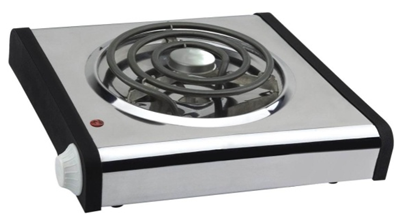
\includegraphics[width = 0.5\linewidth]{electric_stove} 

\end{frame}


\subsection{Duty Cycle}

%Slide-4

\begin{frame}[shrink = 2]

\frametitle{Duty Cycle} \pause

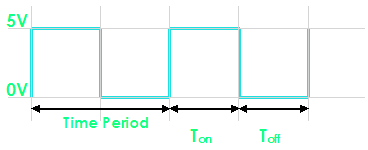
\includegraphics[width = \linewidth]{50_dutycycle} \pause

\begin{enumerate}[$\checkmark$]

\item<+-|alert@+> The signal remains "ON" for some time and  "OFF" for some time.

\item<+-|alert@+> Ton = Time the output remains high.

\item<+-|alert@+> Toff = Time the output remains Low.

\item<+-|alert@+> When output is high the voltage is 5v

\item<+-|alert@+> When output is low the voltage is 0v  

\item<+-|alert@+> Time Period(T) = Ton + Toff

\item<+-|alert@+> Duty Cycle = Ton/(Ton + Toff)

\item<+-|alert@+> Duty Cycle = 50\%

\end{enumerate}

\end{frame}


%Slide-5

\begin{frame}[shrink = 2]

\frametitle{Duty Cycle (Contd..)} \pause

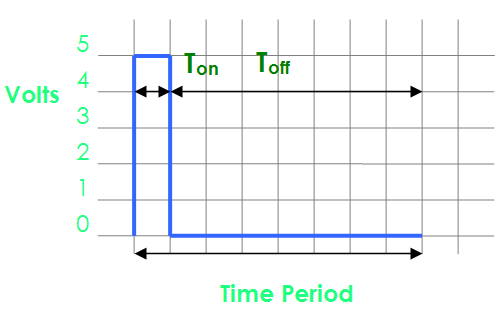
\includegraphics[width = \linewidth]{12_dutycycle} \pause

\begin{enumerate}[$\checkmark$]

\item<+-|alert@+> Ton = Time the output remains high = 1

\item<+-|alert@+> Toff = Time the output remains Low = 7

\item<+-|alert@+> Duty Cycle = 12.5\%

\end{enumerate}

\end{frame}


%Slide-6

\begin{frame}[shrink = 2]

\frametitle{Duty Cycle (Contd..)} \pause

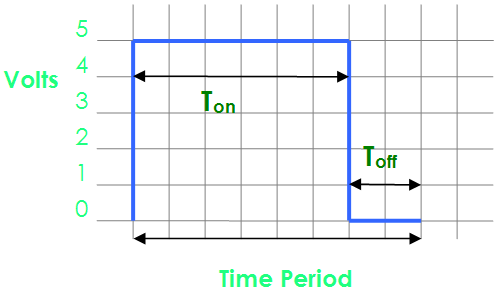
\includegraphics[width = \linewidth]{75_dutycycle} \pause

\begin{enumerate}[$\checkmark$]

\item<+-|alert@+> Ton = Time the output remains high = 6

\item<+-|alert@+> Toff = Time the output remains Low = 2

\item<+-|alert@+> Duty Cycle = 75\%

\end{enumerate}

\end{frame}

\subsection{Motion Control Using Pulse Width Modulation in Firebird V}
\begin{frame}
	\frametitle{Pulse Width Modulation} 
 		\begin{itemize}
 	    \item Pulse width waveform generated for motion control of Firebird V is:
 	    \pause
 	    \centering
 	    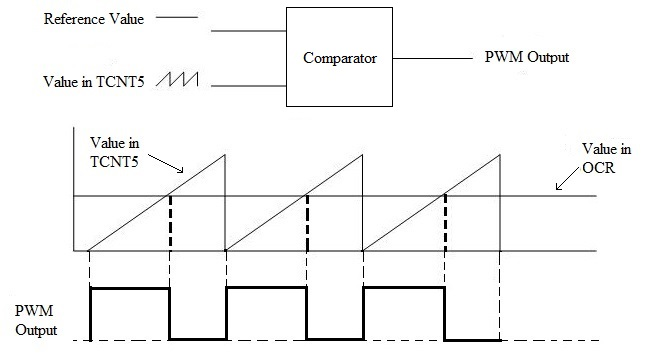
\includegraphics[height=4cm, width=8cm]{PWM}
 	    \end{itemize}
 	    \pause
 		\vfill
 		\begin{itemize}
 	    \item Its generation involves the use of following registers:
 		\pause	 
 		\begin{enumerate} [$\checkmark$]
 			\item <+-|alert@+> Timer/Counter register 5(TCNT5)
 			\item <+-|alert@+> Output Comparator register 5(OCR5A and OCR5B)
 			\item <+-|alert@+> Timer Counter Comparator register(TCCR5A and TCCR5B)
 		\end{enumerate}	
 		\end{itemize}
\end{frame}

%------------------------------------------------

% Start of fourth slide
\section{Registers}
\subsection{Timer/Counter 5(TCNT5)} 
\begin{frame}
	\frametitle{Timer/Counter 5 (TCNT5) }
	\begin{itemize}  % Shows text in bullet point 
		\item <+-|alert@+> The Timer/Counter is a register that increments its value after every clock cycle. 	
		\item <+-|alert@+> The value in the timer/counter is compared with a reference value to generate PWM.
		\item <+-|alert@+> This value depends upon the resolution of Timer.
		\item <+-|alert@+> For example, a 3 bit counter will have 8 values (i.e. 0-7). Its waveform will be seen as follows: 
		\pause
		\vfill
		\begin{center}
			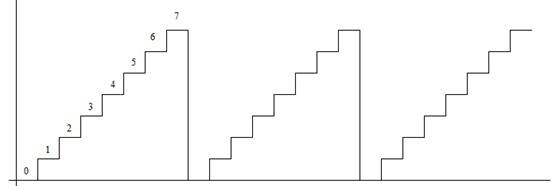
\includegraphics[height=2cm, width=6cm]{PWM2}
		\end{center}
		\item <+-|alert@+> For n-bit counter, maximum value = $2^n - 1$.
		\item <+-|alert@+> The Timer/Counter 5 is a 16 bit register. 
		\item <+-|alert@+> We use it in 8-bit mode, for PWM generation.				
\end{itemize}
\end{frame}

%------------------------------------------------
% Start of fifth slide
\subsection{Output Compare Register 5} 
\begin{frame}
	\frametitle{Output Compare Register (OCR5A, OCR5B and OCR5C)}
	\begin{itemize}
	  \item <+-|alert@+> The value of the Timer/Counter 5 is constantly compared with a reference value.
	  \item <+-|alert@+> This reference value is given in the Output Compare Register(OCR).
	  \item <+-|alert@+>Output Compare Registers associated with Timer 5 for PWM generation:
	  \pause
	  OCR5A, OCR5B and OCR5C.
	  \pause
	  \item <+-|alert@+> For motion control of Firebird V, we use OCR5A and OCR5B registers
	  \item <+-|alert@+> OCR5A is associated with the OC5A pin (PORTL.3). This pin is connected to the enable(EN2) pin of motor driver, which is associated with the left motor.
	  \item <+-|alert@+> Similarly, OCR5B is associated with the OC5B pin (PORTL.4), This pin is connected to the enable(EN1) pin of motor driver, which is associated with the right motor.
	 	  
	\end{itemize}
\end{frame}

%------------------------------------------------
% Start of sixth slide
\subsection{Timer/Counter Control Register (TCCR5A and TCCR5B)} % A subsection can be created just before a set of slides with a common theme to further break down your presentation into chunks
\begin{frame}
\frametitle{Timer/Counter Control Register (TCCR5A and TCCR5B)}
\begin{itemize}
  \item <+-|alert@+> Bits in TCCR5A and TCCR5B registers configure the Timer 5 module for generating PWM
  \item <+-|alert@+> Each bit in these registers determine the kind of signal to be generated.
  \item <+-|alert@+> TCCR5A is a control register and is used to set COM bits and WGM bits.
  \item <+-|alert@+> TCCR5B is also a control register,used to select clock frequency for the Timer 5 and for PWM generation.   
\end{itemize}
\end{frame}

% Start of seventh slide
\subsubsection{TCCR5A} % A subsection can be created just before a set of slides with a common theme to further break down your presentation into chunks
\begin{frame}
	\frametitle{Timer/Counter Control Register 5A(TCCR5A)} \pause
	\begin{tabular}{!{\vrule width 0.8pt}>{\columncolor[gray]{0.9}[0.8\tabcolsep]}c|>{\columncolor[gray]{0.9}[0.8\tabcolsep]}c|>{\columncolor[gray]{0.9}[0.8\tabcolsep]}l|>{\columncolor[gray]{0.9}[0.8\tabcolsep]}c!{\vrule width 1pt}}
		\noalign{\hrule height 1pt}
		\footnotesize Bit & Symbol & Description & Bit Value \\  
		\noalign
		{\hrule height 1pt} 	
		\vspace{1pt} 
	     7 & COM5A1 & Compare Output Mode for Channel A bit 1 & \color{red}  \textbf{1}\color{black} \\
		\vspace{1pt}  
	     6 & COM5A0 & Compare Output Mode for Channel A bit 0 &  0   \\
		\vspace{1pt}  
	     5 & COM5B1 & Compare Output Mode for Channel B bit 1 & \color{red}  \textbf{1}\color{black} \\
		\vspace{1pt}  
		 4 & COM5B0 & Compare Output Mode for Channel B bit 0 &  0 	 \\
		\vspace{1pt} 
		 3 & COM5C1 & Compare Output Mode for Channel C bit 1 & \color{red}  \textbf{1}\color{black} \\
		\vspace{1pt}
		 2 & COM5C0 & Compare Output Mode for Channel C bit 0 &  0 \\
		\vspace{1pt} 
		 1 & WGM11 & Waveform Generation Mode bit 1 &  0 \\
		\vspace{1pt}
		 0 & WGM10 & Waveform Generation Mode bit 0 & \color{red}  \textbf{1}\color{black} \\	
		\noalign{\hrule height 1pt}		
\end{tabular}
		\begin{itemize}
			\item <+-|alert@+> It has 2 types of bits: Compare output mode bit $\&$\ waveform generation mode bit.
			\item <+-|alert@+> Compare Output Mode bits decide the action to be taken when counter(TCNT5) value matches reference value in Output Compare Register(OCR5).
		\end{itemize}
\end{frame}
\begin{frame}
	\frametitle{Timer/Counter Control Register 5A (TCCR5A) (...contd)}
	\begin{itemize}
		\item <+-|alert@+> The Waveform Generation Mode bits are used to generate the type of PWM signal needed.
		\item <+-|alert@+> In the given table:
		\begin{enumerate} [$\checkmark$]
			\item <+-|alert@+> COM5A1 AND COM5A0 bits are used to control the output on left motor. 
			\item <+-|alert@+> COM5B1 and COM5B0 bits are used to control the output on right motor.
		\end{enumerate}
	\end{itemize}
	
\end{frame}	
\begin{frame}
\frametitle{TCCR5A: Compare Output Mode Bits}
\begin{center}
	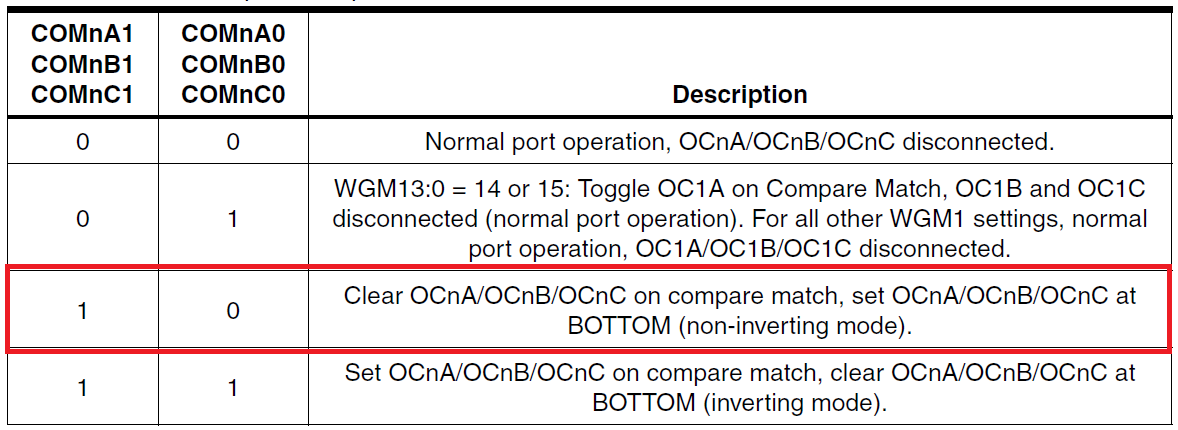
\includegraphics[height=4cm, width=10cm]{com_bits}
\end{center}
	\begin{enumerate}
		\item <+-|alert@+> We are using non-inverting mode for PWM generation.
	\end{enumerate}
\end{frame}		
\begin{frame}
	\frametitle{TCCR5A: Waveform Generation Mode Bits}
	\centering
	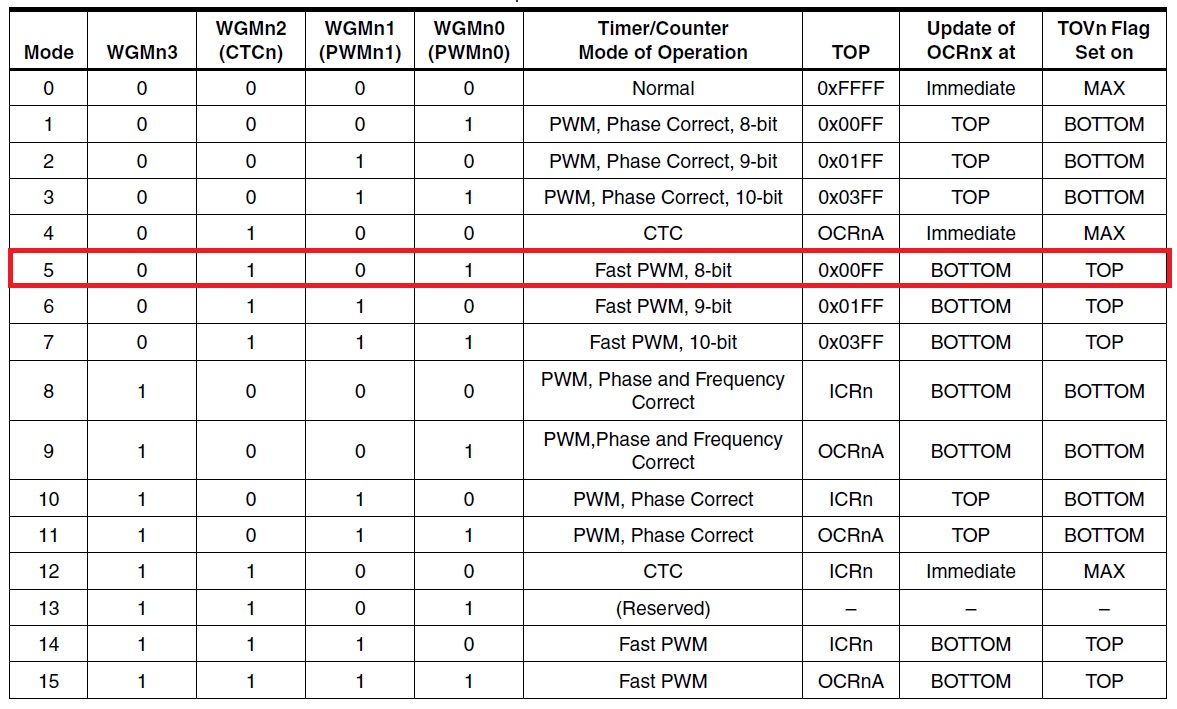
\includegraphics[height=4.5cm, width=9cm]{wg_bits}
	\begin{itemize}
		\item <+-|alert@+> WGM bits determine, type of waveform to be generated. We will be using Fast PWM, 8-bit mode.
	\end{itemize}
\end{frame}
\begin{frame}
	\frametitle{Inverting and Non-inverting mode}
	\centering
	\includegraphics[height = 4.5cm, width = 7cm]{pwm_output}
	\begin{itemize}
		\item <+-|alert@+> There are two modes of pwm waveform generation:
		\item <+-|alert@+> Non-inverting mode and inverting mode 
	\end{itemize}
\end{frame}
\subsubsection{TCCR5B}
\begin{frame}
	\frametitle{Timer/Counter Control Register 5B (TCCR5B)}
	\centering
	\begin{tabular}{!{\vrule width 0.8pt}>{\columncolor[gray]{0.9}[0.8\tabcolsep]}c|>{\columncolor[gray]{0.9}[0.8\tabcolsep]}c|>{\columncolor[gray]{0.9}[0.8\tabcolsep]}l|>{\columncolor[gray]{0.9}[0.8\tabcolsep]}c!{\vrule width 0.8pt}}
		\noalign{\hrule height 0.5pt}
		Bit & Symbol & Description & Bit Value  \\  
		\noalign{\hrule height 1pt} 
		\vspace{2pt} 
		7 & ICNC5 & Input Capture Noise Canceller &  0  \\
		\vspace{2pt}
		6 & ICES5 & Input Capture Edge Select &  0  \\
		\vspace{2pt}
		5 & -- & Reserved Bit &   0 \\
		\vspace{2pt}
		4 & WGM53 & Waveform Generation Mode bit 3 &  0 \\
		\vspace{2pt}
		3 & WGM52 & Waveform Generation Mode bit 2 & \color{red}  \textbf{1}\color{black} \\
		\vspace{2pt}
		2 & CS52 & Clock Select &  0 \\
		\vspace{2pt}
		1 & CS51 & Clock Select & \color{red}  \textbf{1}\color{black}\\
		\vspace{2pt}
		0 & CS50 & Clock Select & \color{red} \textbf{1}\color{black} \\
		\noalign{\hrule height 0.5pt}			
		\end{tabular}	\pause
		\begin{itemize}
			\item In the above Table:
			\pause
			\item <+-|alert@+> Input Capture Noise Canceller and Input Capture Edge Select bits are not being used here. 
			\item <+-|alert@+>WGM bits (WGM52 and WGM53),  are used for PWM generation.
			\item <+-|alert@+> CS52, CS51, CS50 (Clock select) bits are used to select a frequency at which timer/counter Register will increment its value. 
		\end{itemize}
\end{frame}
\begin{frame}
	\frametitle{TCCR5B: Clock Select Bits}
	\begin{center}
		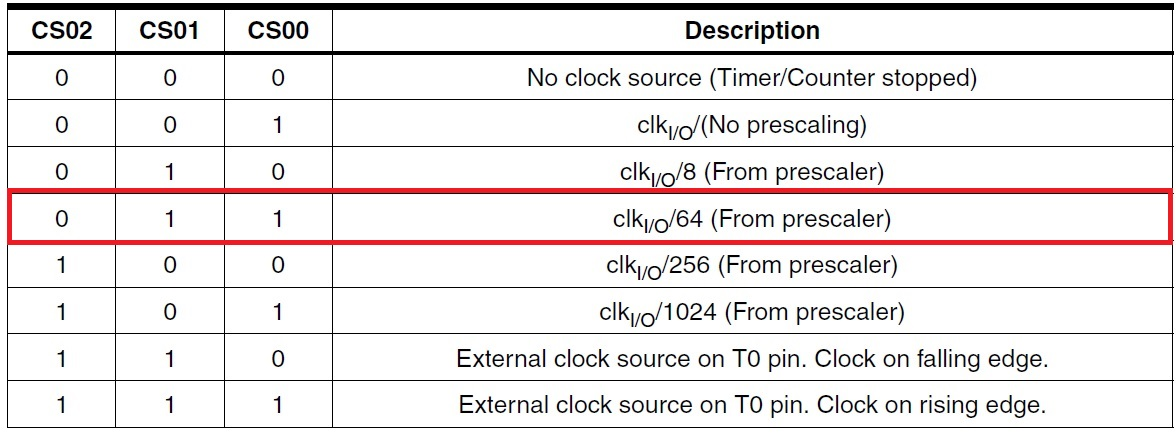
\includegraphics[height=4cm, width=10cm]{cs_bits}
		\begin{itemize}
			\item <+-|alert@+> Prescalar is used to reduce the frequency of the clock, suitable for the type of PWM being generated.
			\item <+-|alert@+> Clock select bits decide the factor with which clock frequency will be divided.
			\item <+-|alert@+> We are using 64 as prescaler so, Clock select bits, we need is 011 .			
		\end{itemize}
	\end{center}
\end{frame}
\begin{frame}
	\frametitle{PWM Mode selection}
	\begin{itemize}
		\item <+-|alert@+> Component frequency = $\dfrac{f_{clk_{I/O}}} {N\ x\ prescaler} ..............equation(1)$	
	    \item <+-|alert@+> Here the component is DC motor whose frequency is 1000Hz
		\item <+-|alert@+> $Clock frequency(f_{clk_{I/O}})  = 14745600Hz$
		
		\item <+-|alert@+> Since we are using PWM in 8 bit mode N = $2^8 $= 256
		
		\item <+-|alert@+> Putting all the above values in equation (1), we get
		
		\item <+-|alert@+> 1000 =
		$\dfrac{14745600}{2^8\ x\ prescaler}$
		
		\item  <+-|alert@+>  1000 = $\dfrac{14745600}{256\ x\ prescaler}$
		
		\item <+-|alert@+> prescaler = $\dfrac{14745600}{256\ x\ 1000}$
		\item <+-|alert@+> prescaler = 57.6
		
		\item <+-|alert@+> Closest value to 57.6 is 64. So, we chose 64 as a prescaler value in 8-bit Fast PWM mode.
		
	\end{itemize}
\end{frame}
\section{Summary}
\begin{frame}
\frametitle{Summary}
 \begin{itemize}
 	\item <+-|alert@+> In order to use Fast PWM mode to control dc motors of Firebird V. We have to initialize following registers.
 	\item
 	\pause
 	TCNT5H  = 0xFF 
 	\item
 	\pause
 	TCNT5L = 0x00 
	\item
	\pause
	TCCR5A  = 0xA9
	\item
	\pause 
	TCCR5B = 0x0B 
	\item
	\pause 
	OCR5AH = 0x00 
	\item
	\pause 
	OCR5AL = 0xFF
	\item
	\pause 
	OCR5BH = 0x00 
	\item
	\pause
	OCR5BL = 0xFF
	
\end{itemize}
\end{frame}
\section{Program}

%Slide-20

\begin{frame}[shrink = 4,fragile]
\frametitle{Syntax for C-Program} \pause
\framesubtitle{PWM Initialization}
\begin{block}<1->{Port Pin Config}	\pause
\begin{semiverbatim}
\scriptsize{
void motion_pin_config (void) \color{green} //Configure Pins as Output\color{black}
\{

Port A for motion control and Port L for Velocity Control must be defined Output
\} }
\end{semiverbatim}
\end{block} \pause
\begin{block}<1->{PWM Initialization}	\pause
\begin{semiverbatim}
\scriptsize{
void timer5_init()	\color{green} //Set Register Values for starting Fast 8-bit PWM  \color{black}
\{
TCCR5A =  
\ \ \	TCCR5B =
\ \ \	TCNT5H = 0xFF; 
\ \ \	TCNT5L = 0x00; 
\ \ \	OCR5AH = 0x00;
\ \ \ OCR5AL = 0xFF;
\ \ \	OCR5BH = 0x00;
\ \ \ OCR5BL = 0xFF;
\} }
\end{semiverbatim}
\end{block} 
\end{frame}
%Slide-21
\begin{frame}[shrink = 2,fragile]
\frametitle{Syntax for C-Program} \pause
\framesubtitle{Program}
\begin{block}<1->{Main Program}	\pause
\begin{semiverbatim}
\scriptsize{
int main(void)
\{
\ \		init_devices(); 
\ \		forward();
\ \		while(1)
\ \		\{
\ \ \ \			velocity(100,100);
\ \ \ \			_delay_ms(500);
\ \ \ \			velocity(0,255);
\ \ \ \			_delay_ms(500);
\ \		\}
\}
}
\end{semiverbatim}
\end{block} \pause
\begin{block}<1->{Velocity Function}	\pause
\begin{semiverbatim}
\scriptsize{
void velocity (unsigned char left_motor, unsigned char right_motor)	
\{
OCR5AL = (unsigned char)left_motor;
\ \ \	OCR5BL = (unsigned char)right_motor;
\}} 
\end{semiverbatim}
\end{block} 
\end{frame}
\begin{frame}
	\centering
	\vspace{2cm}	
	\textbf{\Huge Thank You!} \\[60pt]
\end{frame}
\end{document}
